\documentclass[11pt,a4paper]{article}
\usepackage[margin=2.1cm]{geometry}
\usepackage{lmodern}
\usepackage[T1]{fontenc}
\usepackage{amsmath,amssymb,bm,mathtools}
\usepackage{booktabs,array,tabularx}
\usepackage{enumitem}
\usepackage{xcolor}
\usepackage{microtype}
\usepackage{tikz}
\usetikzlibrary{arrows.meta}
\usepackage[colorlinks=true,linkcolor=blue!55!black,urlcolor=blue!55!black]{hyperref}
\setlength{\parindent}{0pt}\setlength{\parskip}{6pt plus 2pt minus 1pt}
\allowdisplaybreaks

\newcommand{\vect}[1]{\bm{#1}}
\newcommand{\mat}[1]{\bm{#1}}
\newcommand{\T}{^{\mathsf{T}}}
\newcommand{\Real}{\mathbb{R}}
\newcommand{\diag}{\operatorname{diag}}
\DeclareMathOperator{\blkdiag}{blkdiag}
\newcommand{\Rot}{\mat{R}}
\newcommand{\dU}{\Delta\vect{U}}
\newcommand{\du}{\Delta\vect{u}}
\newcommand{\Ts}{T_s}
\newcommand{\Np}{N_p}
\newcommand{\Nc}{N_c}
\newcommand{\Qbar}{\bar{\mat{Q}}}
\newcommand{\Rbar}{\bar{\mat{R}}}
\newcommand{\ones}{\vect{1}}

\newcommand{\course}{\textbf{\textcolor{blue!60!black}{Course.}}\ }
\newcommand{\ours}{\textbf{\textcolor{green!45!black}{Ours.}}\ }
\newcommand{\why}{\textbf{\textcolor{red!60!black}{Why it differs.}}\ }
\newcommand{\tcheck}{\textbf{Check.}\ }

\title{From the course MPC to the docking MPC\\[4pt]\large A step-by-step bridge, with every divergence named}
\author{}
\date{9 October 2026}

\begin{document}
\maketitle
\vspace{-1.5em}

\section*{How to read this}
Every step below has the same four parts. \course what Section~5 of the MECHENG~724 notes does, with the notes' own equation. \ours what the docking controller does. \why the reason for any difference, and what would go wrong without it. \tcheck which test in \texttt{matlab/tests} verifies that step of your implementation. The notes are cited by their section numbers (5.3.2, 5.4.1, \ldots); the design document \texttt{docking\_formulation.pdf} by ``DD~4.x''. A worked numerical tick with small horizons runs through the whole document so you can follow the matrices by hand.

There are only four places where the docking MPC leaves the notes, and each is forced by the problem rather than by taste:
\begin{enumerate}[nosep]
  \item the plant is nonlinear, so the matrices are rebuilt every tick (\emph{successive linearisation});
  \item the outputs have mixed units, so the output error is weighted (\emph{Bryson's rule});
  \item the actuator limits are per wheel, so the amplitude constraint goes through the mecanum kinematics;
  \item two of the constraints are on outputs, so they are soft, with a slack variable, exactly as 5.4.1 says they usually must be.
\end{enumerate}
Everything else, the augmented model, the prediction matrices, the cost, the closed-form solution, the receding horizon, the constraint assembly and the quadratic programme, is the notes' material applied with $m = 3$ inputs and $p = 3$ outputs.

\section{The big picture}
The schematic on page~1 of Section~5 has a plant model and an optimiser inside the MPC box, a reference coming in, and a state estimator feeding estimated states back. Ours is that schematic with names filled in:
\begin{center}
\small
\begin{tabularx}{\linewidth}{l >{\raggedright\arraybackslash}p{4.0cm} X}
\toprule
Schematic box & Course & Docking controller \\
\midrule
Plant model & given $(A, B, C)$, discrete LTI & kinematics of the chassis in the target frame, linearised each tick (DD~4.1--4.2) \\
Manipulated variables & $\vect u(k)$ & body-velocity command $[u_b;\ v_b;\ r_b]$, converted to wheel speeds after the tick \\
Reference & $y_r$ constant & docked pose $(0,0,0)$, or the standoff pose during the approach (DD~4.7) \\
State estimator & ``estimated states'' & the docking EKF, which supplies the pose and the velocity (DD~3) \\
Optimiser & \texttt{quadprog} & \texttt{quadprog}, same call, one extra variable for the slack \\
\bottomrule
\end{tabularx}
\end{center}

\textbf{A picture to keep.} The receding horizon of 5.2 and 5.3.5, with one addition: the dot at the start of each horizon is where the matrices are rebuilt. Everything inside a horizon is the course's linear MPC; what moves between horizons is the linearisation point.
\begin{center}
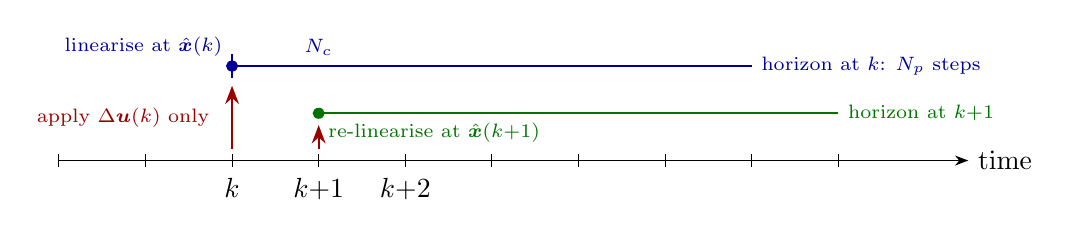
\begin{tikzpicture}[>=Stealth, x=1.1cm, y=1cm]
  \draw[->] (0,0) -- (10.5,0) node[right] {time};
  \foreach \k in {0,...,9} { \draw (\k,-0.08) -- (\k,0.08); }
  \node[below] at (2,-0.1) {$k$}; \node[below] at (3,-0.1) {$k{+}1$}; \node[below] at (4,-0.1) {$k{+}2$};
  \draw[thick, blue!60!black] (2,1.2) -- (8,1.2);
  \draw[thick, blue!60!black] (2,1.2) -- (4,1.2) node[midway, above, font=\scriptsize] {$\Nc$};
  \node[right, font=\scriptsize, blue!60!black] at (8,1.2) {horizon at $k$: $\Np$ steps};
  \fill[blue!60!black] (2,1.2) circle (0.07) node[above left, font=\scriptsize] {linearise at $\hat{\vect x}(k)$};
  \draw[blue!60!black, thick] (2,1.05) -- (2,1.35);
  \draw[thick, green!45!black] (3,0.6) -- (9,0.6);
  \fill[green!45!black] (3,0.6) circle (0.07) node[below right, font=\scriptsize] {re-linearise at $\hat{\vect x}(k{+}1)$};
  \node[right, font=\scriptsize, green!45!black] at (9,0.6) {horizon at $k{+}1$};
  \draw[->, red!60!black, thick] (2,0.15) -- (2,0.95);
  \node[red!60!black, font=\scriptsize, anchor=east] at (1.85,0.55) {apply $\du(k)$ only};
  \draw[->, red!60!black, thick] (3,0.15) -- (3,0.45);
\end{tikzpicture}
\end{center}

\section{Step 1: the plant model, and why it is rebuilt every tick}
\course 5.3.2 starts from a discrete linear time-invariant model
\begin{equation}
\vect x(k+1) = \mat A\vect x(k) + \mat B\vect u(k),\qquad \vect y(k) = \mat C\vect x(k),
\end{equation}
with constant matrices, and remarks that $\mat D$ is dropped because the current input cannot affect the current output.

\ours The thing being controlled is the pose $\vect x_c = [x;\ y;\ \theta]$ of the chassis in the target frame, driven by the body-velocity command. The continuous kinematics are nonlinear because the command is in body axes and the pose in target axes:
\begin{equation}
\dot x = u_b\cos\theta - v_b\sin\theta,\qquad \dot y = u_b\sin\theta + v_b\cos\theta,\qquad \dot\theta = r_b.
\end{equation}
Two course tools turn this into the form 5.3.2 wants. Discretisation (2.5), Euler at the MPC period $\Ts$:
\begin{equation}
\vect x_c(k+1) = \vect f_c(\vect x_c,\vect u) = \vect x_c + \Ts\!\begin{bmatrix}u_b\cos\theta - v_b\sin\theta\\ u_b\sin\theta + v_b\cos\theta\\ r_b\end{bmatrix}\!.
\end{equation}
Jacobian linearisation (6.2), but about the \emph{current estimate and the last command} $(\bar{\vect x}, \bar{\vect u}) = (\hat{\vect x}_c(k), \vect u(k-1))$ instead of a fixed equilibrium:
\begin{gather}
\mat A_k = \left.\frac{\partial\vect f_c}{\partial\vect x_c}\right|_{\bar{\vect x},\bar{\vect u}}
= \mat I_3 + \Ts\begin{bmatrix}0 & 0 & -(\bar u_b\sin\bar\theta + \bar v_b\cos\bar\theta)\\ 0 & 0 & \bar u_b\cos\bar\theta - \bar v_b\sin\bar\theta\\ 0 & 0 & 0\end{bmatrix},\\
\mat B_k = \left.\frac{\partial\vect f_c}{\partial\vect u}\right|_{\bar{\vect x},\bar{\vect u}}
= \Ts\begin{bmatrix}\cos\bar\theta & -\sin\bar\theta & 0\\ \sin\bar\theta & \cos\bar\theta & 0\\ 0 & 0 & 1\end{bmatrix},
\qquad \mat C = \mat I_3.
\end{gather}
The only nonlinear entries are the heading column of $\mat A_k$, which says how a heading change redirects the current command, and the rotation inside $\mat B_k$, which says which way in the target frame a body command pushes.

\why The course's constant $(\mat A, \mat B)$ would be the linearisation at a single equilibrium, 6.2's $(\vect x^*, \vect u^*)$. The docked pose with zero command is such an equilibrium, and at it $\mat B = \Ts\mat I$: the three axes decouple completely. That model is accurate only while the heading stays near zero. During the approach the heading can be $15^\circ$ or more, where the fixed-point model mis-assigns a quarter ($\sin 15^\circ = 0.26$) of a forward command to the lateral axis. Re-linearising at the current estimate every tick keeps the model accurate wherever the robot is, at the cost of rebuilding the matrices every tick. This is the same Taylor-series idea as 6.2 with a moving expansion point, and it is the one new idea in the whole controller.

\textbf{The affine term.} Linearising about a point that is not an equilibrium leaves a constant: $\vect x_c(k+1)\approx\mat A_k\vect x_c(k) + \mat B_k\vect u(k) + \vect c_k$ with $\vect c_k = \vect f_c(\bar{\vect x},\bar{\vect u}) - \mat A_k\bar{\vect x} - \mat B_k\bar{\vect u}$. The course never meets this because its model is linear. It disappears in Step~2.

\textbf{Worked tick.} With $\Ts = 0.05$~s, at zero heading and a forward command of $0.2$~m/s,
\begin{equation}
\mat A_k = \begin{bmatrix}1 & 0 & 0\\ 0 & 1 & 0.01\\ 0 & 0 & 1\end{bmatrix},\qquad
\mat B_k = 0.05\,\mat I_3 .
\end{equation}
The entry $0.01 = \Ts\bar u_b$ says: a heading error of one radian, held for one tick while driving forward at $0.2$~m/s, moves the robot $10$~mm sideways. At $15^\circ$ heading with command $[0.2;\ 0.05;\ 0]$ the same matrices are
\begin{equation}
\mat A_k = \begin{bmatrix}1 & 0 & -0.0050\\ 0 & 1 & 0.0090\\ 0 & 0 & 1\end{bmatrix},\qquad
\mat B_k = \begin{bmatrix}0.0483 & -0.0129 & 0\\ 0.0129 & 0.0483 & 0\\ 0 & 0 & 0.05\end{bmatrix},
\end{equation}
where $\mat B_k$ is $0.05\,\Rot(15^\circ)$ in its top-left block.

\tcheck \texttt{test\_mpc\_linearisation} differences your own $\vect f_c$ numerically and compares.

\section{Step 2: the augmented incremental model}
\course 5.3.2 differences the state equation to get $\Delta\vect x(k+1) = \mat A\Delta\vect x(k) + \mat B\du(k)$, writes the output at the next step as $\vect y(k+1) = \mat C\mat A\Delta\vect x(k) + \vect y(k) + \mat C\mat B\du(k)$, and stacks the two into
\begin{equation}
\vect x_p(k) = \begin{bmatrix}\Delta\vect x(k)\\ \vect y(k)\end{bmatrix},\qquad
\mat A_p = \begin{bmatrix}\mat A & \mat 0\\ \mat C\mat A & \mat I\end{bmatrix},\qquad
\mat B_p = \begin{bmatrix}\mat B\\ \mat C\mat B\end{bmatrix},\qquad
\mat C_p = \begin{bmatrix}\mat 0 & \mat I\end{bmatrix}.
\end{equation}
The class exercise asks where the extra eigenvalues sit: the augmented matrix has the eigenvalues of $\mat A$ plus $p$ eigenvalues at $1$, the integrators that give the controller its integral action.

\ours Identical, with $\mat C = \mat I_3$ so that $\mat C\mat A = \mat A_k$ and $\mat C\mat B = \mat B_k$:
\begin{equation}
\vect x_p(k) = \begin{bmatrix}\Delta\vect x_c(k)\\ \vect x_c(k)\end{bmatrix}\in\Real^6,\qquad
\mat A_p = \begin{bmatrix}\mat A_k & \mat 0_{3\times3}\\ \mat A_k & \mat I_3\end{bmatrix},\qquad
\mat B_p = \begin{bmatrix}\mat B_k\\ \mat B_k\end{bmatrix},\qquad
\mat C_p = \begin{bmatrix}\mat 0_{3\times3} & \mat I_3\end{bmatrix}.
\end{equation}
Since $\mat A_k$ is the identity plus terms of order $\Ts$, all six eigenvalues of $\mat A_p$ sit at $1$: the plant is three integrators (velocity command to position) and the augmentation adds three more. With $r_w = 0$ the solution would be the dead-beat one of Example~5.3, which here asks for velocity increments far beyond what the wheels can deliver; Step~4 shows the numbers.

\textbf{Why the affine term vanishes.} Differencing consecutive steps of $\vect x_c(k+1) = \mat A_k\vect x_c(k) + \mat B_k\vect u(k) + \vect c_k$, with the matrices frozen over the horizon, subtracts $\vect c_k$ from itself. So the incremental model is exactly 5.3.2's, and successive linearisation costs no extra term. This is the single most useful property of the course's $\Delta\vect u$ formulation for a nonlinear plant.

\textbf{The initial increment.} The course forms $\Delta\vect x(k) = \vect x(k) - \vect x(k-1)$ by differencing two measured states (Example~5.4 does exactly this by hand). Differencing two noisy pose estimates $50$~ms apart would be a very poor velocity. We have an estimator that carries velocity as a state, so
\begin{equation}
\Delta\vect x_c(k) = \Ts\begin{bmatrix}\hat v_x\\ \hat v_y\\ r_k\end{bmatrix},\qquad \vect x_c(k) = \begin{bmatrix}\hat x\\ \hat y\\ \hat\theta\end{bmatrix},
\end{equation}
with the yaw rate straight from the gyro. Feeding the \emph{measured} velocity here is also what gives the controller its disturbance rejection: if the wheels slip and deliver less than commanded, the increment state says so and the optimiser compensates.

\textbf{Worked tick.} From the zero-heading matrices above,
\begin{equation}
\mat A_p = \left[\begin{array}{ccc|ccc}
1 & 0 & 0 & 0 & 0 & 0\\ 0 & 1 & 0.01 & 0 & 0 & 0\\ 0 & 0 & 1 & 0 & 0 & 0\\ \hline
1 & 0 & 0 & 1 & 0 & 0\\ 0 & 1 & 0.01 & 0 & 1 & 0\\ 0 & 0 & 1 & 0 & 0 & 1\end{array}\right],\qquad
\mat B_p = \begin{bmatrix}0.05\,\mat I_3\\ 0.05\,\mat I_3\end{bmatrix}.
\end{equation}

\section{Step 3: prediction over the horizon}
\course 5.3.3 stacks the predicted outputs $\vect y(k_i+1|k_i),\ldots,\vect y(k_i+\Np|k_i)$ into $\vect Y$ and the future increments $\du(k_i),\ldots,\du(k_i+\Nc-1)$ into $\dU$, and gets
\begin{equation}
\vect Y = \mat F\vect x_p(k_i) + \mat\Phi\dU,\qquad
\mat F = \begin{bmatrix}\mat C_p\mat A_p\\ \mat C_p\mat A_p^2\\ \vdots\\ \mat C_p\mat A_p^{\Np}\end{bmatrix},\qquad
\mat\Phi = \begin{bmatrix}\mat C_p\mat B_p & \mat 0 & \cdots\\ \mat C_p\mat A_p\mat B_p & \mat C_p\mat B_p & \cdots\\ \vdots & \vdots & \ddots\\ \mat C_p\mat A_p^{\Np-1}\mat B_p & \mat C_p\mat A_p^{\Np-2}\mat B_p & \cdots\end{bmatrix},
\end{equation}
with the last column of $\mat\Phi$ stopping at $\mat C_p\mat A_p^{\Np-\Nc}\mat B_p$ because increments beyond $\Nc$ are zero. \texttt{mpcgain.m} builds exactly these for a scalar system.

\ours The same two matrices, with every scalar entry replaced by a $3\times3$ block: $\mat F$ is $3\Np\times 6$ and $\mat\Phi$ is $3\Np\times 3\Nc$. The notes say in 5.3.4 that the MIMO extension ``is straightforward following similar steps'', and it is: the block in row $i$, column $j$ of $\mat\Phi$ is $\mat C_p\mat A_p^{\,i-j}\mat B_p$ for $i\ge j$ and zero above the diagonal.

\why Nothing differs except dimension, and one consequence of Step~1: because $\mat A_p, \mat B_p$ change every tick, $\mat F$ and $\mat\Phi$ are rebuilt every tick. For $\Np = 40$, $\Nc = 10$ that is a few thousand multiplications, well inside the $50$~ms period.

\textbf{Worked tick}, with $\Np = 4$, $\Nc = 2$ so the matrices fit on the page. At zero heading the three axes decouple and the $x$-axis rows of $\mat F$ and $\mat\Phi$, picked out with their $x$ columns, are
\begin{equation}
\mat F_x = \begin{bmatrix}1 & 1\\ 2 & 1\\ 3 & 1\\ 4 & 1\end{bmatrix},\qquad
\mat\Phi_x = \begin{bmatrix}0.05 & 0\\ 0.10 & 0.05\\ 0.15 & 0.10\\ 0.20 & 0.15\end{bmatrix}.
\end{equation}
Compare Example~5.2: there $a = 0.8$, $b = 0.1$ gave a first column of $\mat F$ that saturated ($0.8, 1.44, 1.95, \ldots$) and a $\mat\Phi$ whose entries grew by shrinking amounts. Here $a = 1$ and $b = \Ts$, an integrator, so the first column of $\mat F_x$ counts steps and $\mat\Phi_x$ grows linearly: a velocity increment applied now moves the position by $\Ts$ more at every later step. The full $12\times 6$ matrices only add the $0.01$ coupling from heading into $y$ (entries $0.03, 0.06, 0.10$ in $\mat F$ and $0.0005, 0.0015, 0.003$ in $\mat\Phi$), which is the heading column of $\mat A_k$ propagating.

\tcheck \texttt{test\_mpc\_prediction} compares your $\mat F, \mat\Phi$ against brute-force stepping of the augmented model, and the $x$-axis sub-blocks against \texttt{mpcgain.m} itself, which must agree to machine precision.

\section{Step 4: the cost function and the unconstrained solution}
\course 5.3.4 writes
\begin{equation}
J = (\vect Y_r - \vect Y)\T(\vect Y_r - \vect Y) + \dU\T\Rbar\dU,\qquad \Rbar = r_w\mat I,
\end{equation}
with $\vect Y_r$ the set-point repeated $\Np$ times, substitutes the prediction, differentiates, and finds
\begin{equation}
\dU = \big(\mat\Phi\T\mat\Phi + \Rbar\big)^{-1}\mat\Phi\T\big(\vect Y_r - \mat F\vect x_p(k_i)\big).
\end{equation}
Example~5.3 then shows $r_w = 0$ giving a dead-beat answer and $r_w = 10$ a sluggish one.

\ours Two weighting matrices appear:
\begin{equation}
J = (\vect Y_r - \vect Y)\T\Qbar(\vect Y_r - \vect Y) + \dU\T\Rbar\dU,\qquad
\Qbar = \mat I_{\Np}\otimes\mat Q_y,\quad
\Rbar = r_w\,\mat I_{\Nc}\otimes\mat R_u,
\end{equation}
and the same derivative gives the same solution with $\mat\Phi\T\mat\Phi$ replaced by $\mat\Phi\T\Qbar\mat\Phi$ and $\mat\Phi\T$ by $\mat\Phi\T\Qbar$:
\begin{equation}
\dU^\star = \big(\mat\Phi\T\Qbar\mat\Phi + \Rbar\big)^{-1}\mat\Phi\T\Qbar\big(\vect Y_r - \mat F\vect x_p(k)\big).
\end{equation}
The weights come from Bryson's rule in 3.4,
\begin{equation}
\mat Q_y = \diag\!\big(1/y_{\mathrm{tol}}^2,\ 1/y_{\mathrm{tol}}^2,\ 1/\theta_{\mathrm{tgt}}^2\big),\qquad
\mat R_u = \diag\!\big(1/\Delta u_{\max,1}^2,\ 1/\Delta u_{\max,2}^2,\ 1/\Delta u_{\max,3}^2\big),
\end{equation}
so that a position error equal to the coupler tolerance, a heading error equal to the internal heading target, and an increment equal to its limit each cost one unit. The scalar $r_w$ is then the course's knob, scaling the whole increment term.

\why The course's unit weight on the output error is fine for one output. Ours are two metres and one angle in radians, and the acceptable errors are $80$~mm and $1.5^\circ = 0.026$~rad at full scale. With unit weights the controller would spend effort on heading only once the heading error was comparable in raw number to a position error, which is physically meaningless. Bryson's rule normalises each error by what counts as ``one unit of bad''. The kronecker product $\mat I_{\Np}\otimes\mat Q_y$ just repeats the $3\times3$ weight down the diagonal, once per predicted step, exactly as $\vect Y_r$ repeats the set-point.

\textbf{Worked tick.} Full-scale weights, $r_w = 1$:
\begin{equation}
\mat Q_y = \diag(156,\ 156,\ 1459),\qquad \mat R_u = \diag(4444,\ 4444,\ 1600).
\end{equation}
Take the robot one metre out, $5$~cm to the left, heading zero, moving forward at $0.2$~m/s, so $\vect x_p = [0.01;\ 0;\ 0;\ -1;\ 0.05;\ 0]$, reference zero. The unconstrained solution over $\Nc = 2$ is
\begin{equation}
\dU^\star = \begin{bmatrix}0.0170 & -0.0009 & -0.0000\\ 0.0102 & -0.0005 & -0.0000\end{bmatrix}\ \text{(one row per step)},
\qquad
\vect u(k) = \vect u(k-1) + \du(k) = \begin{bmatrix}0.217\\ -0.0009\\ -0.0000\end{bmatrix},
\end{equation}
and the predicted $x$ over the four steps is $-0.989, -0.978, -0.966, -0.955$~m. Even this gentle tick asks for a forward increment of $0.017$~m/s, above the acceleration limit of $\Ts a_{\max} = 0.015$~m/s per tick. With the position weights on the internal target instead, nine times heavier ($\mat Q_y = \diag(1372, 1372, 1459)$), the same tick asks for $0.145$~m/s, ten times the limit, and a command of $0.345$~m/s above the speed cap: the dead-beat tendency of Example~5.3 with $r_w = 0$. Step~6 is what keeps either inside the actuator.

\textbf{Why the position weight uses the tolerance and the heading weight the internal target.} The obvious choice is one level for all three outputs, and it was the first choice. It fails for a reason that only the closed loop shows. The heading column of $\mat A_k$ makes the heading a lateral actuator through the forward speed (one radian of heading at $0.3$~m/s is $0.3$~m/s of lateral drift), a double-integrator path that runs through the wheel lag the kinematic model does not contain. With the lateral error weighted on the internal target the optimiser steers with the heading: on the demonstrator the heading swung by $\pm 20^\circ$ during the approach and the yaw-rate command alternated at its increment limit. With the lateral error weighted on the tolerance it crabs instead, which is what a mecanum chassis is for. Accuracy at the dock does not suffer, because the steady-state error comes from the integral action of Step~2 and not from the weight: the lateral error at docking stays below $4$~mm on both variants in the closed-loop tests. DD~4.5.

\tcheck \texttt{test\_mpc\_unconstrained} removes the limits and compares your \texttt{mpc\_step} with this closed form.

\section{Step 5: receding horizon and the explicit gains}
\course 5.3.5 applies only the first element of $\dU$, moves one step, measures, and solves again. 5.3.6 pulls the first row out of the closed form to write $\du(k_i) = \mat K_y y_r - \mat K_{\mathrm{mpc}}\vect x_p(k_i)$ and draws the block diagram with the integrator $z/(z-1)$ and the differencer $(z-1)/z$.

\ours Identical, with the first \emph{block} of three entries applied, as the notes say for MIMO. The gains $\mat K_y$ and $\mat K_{\mathrm{mpc}} = [\mat K_x\ \ \mat K_y]$ exist in the same way, as the first three rows of $(\mat\Phi\T\Qbar\mat\Phi + \Rbar)^{-1}\mat\Phi\T\Qbar(\cdot)$, but they change every tick with $\mat F, \mat\Phi$.

\why Only Step~1 again: the gains are time-varying because the linearisation is. They still matter for two reasons. They are the fallback if a solver is ever unavailable, a $3\times6$ gain times the state followed by saturation. And near the dock, where the heading stays near zero and the matrices stop changing, they settle to constants, so the final approach is in effect the course's LTI controller, which is a useful thing to say in the report.

\section{Step 6: constraints}
\course 5.4.1 lists three types: (i) on the increments $\Delta u_{\min}\le\du\le\Delta u_{\max}$, (ii) on the amplitudes $u_{\min}\le\vect u\le u_{\max}$ through the accumulation $\vect U = \mat C_1\vect u(k_i-1) + \mat C_2\dU$, and (iii) on outputs $y_{\min}\le\vect y\le y_{\max}$ through the prediction, with the warning that output constraints may be infeasible and are usually made soft with a slack $s_v\ge 0$. 5.4.2 rewrites each two-sided limit as two one-sided rows and stacks them into $\mat M\dU\le\vect\gamma$ with $4m\Nc + 2p\Np$ rows.

\ours Every one of the three types is used, and the mapping is:
\begin{center}
\small
\begin{tabularx}{\linewidth}{l X l l}
\toprule
Course type & Physical limit here & Rows & Hard or soft \\
\midrule
(i) increments & acceleration limit (anti-slip): $|\du|\le\Ts[a_{\max};\ a_{\max};\ \alpha_{\max}]$ & $6\Nc$ & hard \\
(ii) amplitudes & speed cap $|u_b|+|v_b|\le v_{\max}$ (four facets), lowered in the final approach, and $|r_b|\le r_{\max}$ & $6\Nc$ & hard \\
(ii) through a map & wheel speeds $|\mat J^{-}\vect u|\le\omega_{\max}$, four wheels & $8\Nc$ & hard \\
(iii) output & no penetration past the contact band, $x(k+j)\le x_{\max}$ & $\Np$ & soft \\
(iii) output & heading corridor $|\theta(k+j)|\le\theta_{\max}$, marker stays in view & $2\Np$ & soft \\
\bottomrule
\end{tabularx}
\end{center}
The accumulation matrices are the course's, block form: $\mat C_1 = \ones_{\Nc}\otimes\mat I_3$, $\mat C_2 = \mat L_{\Nc}\otimes\mat I_3$ with $\mat L$ lower-triangular ones.

\why Four things to explain.

\emph{The shape of the speed cap.} The notes' amplitude limit is a box, $u_{\min}\le\vect u\le u_{\max}$ on each input. A box on the two body velocities is $41\,\%$ faster along its diagonal than along its axes, and the optimiser finds this: on the demonstrator it yawed the body to the edge of the heading corridor for the whole approach, to drive on the diagonal. The cap is therefore the L1 bound $|u_b|+|v_b|\le v_{\max}$, written as its four facets $\pm u_b\pm v_b\le v_{\max}$, four rows per step. It bounds the speed norm in every direction, and it is the shape of the wheel-speed limit at zero yaw rate, $|u_b|+|v_b|+L|r_b|\le R_w\omega_{\max}$, so the chassis is fastest along its own axes and has no reason to yaw. The yaw rate keeps its two box rows. Still type (ii), still linear in $\dU$ through $\mat C_1$ and $\mat C_2$, still six rows per step.

\emph{The wheel rows.} The notes only have box limits on $\vect u$. Our actuators are four motors, each with a speed limit, and the mecanum inverse kinematics $\vect\omega = \mat J^{-}\vect u$ is a constant linear map, so the wheel limits are box limits on $\mat J^{-}\vect U$: still linear in $\dU$, still type (ii), eight rows per step instead of six. This is how the kinematics enter the controller. The decision variables stay in body velocity because the fourth wheel degree of freedom only scrubs the rollers and the kinematic model cannot see it.

\emph{Why the output rows are soft, and how the slack works.} 5.4.1 says output constraints ``may violate constraints of types (i) and (ii)'' and ``can make the optimisation problem infeasible''. That is not hypothetical here. At contact the estimate can sit a few millimetres past the plane, through wheel lag or estimation noise, and no increment sequence inside the acceleration limit can bring the predicted $x$ back below the plane at the first steps, so a hard row has no feasible point and \texttt{quadprog} returns nothing. The remedy is the notes' $s_v$: append one slack $s\ge 0$ to the decision vector, subtract it from every soft row so that $x(k+j) - s\le x_{\max}$, and penalise it in the cost. In the QP this means
\begin{equation}
\vect z = \begin{bmatrix}\dU\\ s\end{bmatrix},\qquad
\mat E_{\mathrm{ext}} = \begin{bmatrix}\mat E & \vect 0\\ \vect 0\T & \epsilon\end{bmatrix},\qquad
\vect f_{\mathrm{ext}} = \begin{bmatrix}\vect f\\ \rho_s\end{bmatrix},\qquad
\mat M_{\mathrm{ext}} = \begin{bmatrix}\mat M_{\mathrm{hard}} & \vect 0\\ \mat M_{\mathrm{soft}} & -\ones\end{bmatrix},
\end{equation}
with the lower bound $s\ge 0$ passed to the solver. The penalty is \emph{linear}, $\rho_s s$, on purpose: a linear penalty larger than any constraint multiplier is exact, meaning $s$ is zero whenever the hard constraint can be met, whereas a quadratic penalty always trades a small violation against tracking. Because the multipliers scale with $\mat Q_y$, so must $\rho_s$; the parameter file sets it to $100\,\Np\max(\mat Q_y)$.

\emph{Why a contact band.} With the plane at first contact, the controller bounces: the lag carries the robot a millimetre past the plane, the exact penalty demands maximum reverse, the tracking cost drives it forward again, and the dock criterion never sees a slow robot. A coupler needs a few millimetres of engagement travel anyway, so the constraint plane sits at the end of that travel, $x_{\max} = 10$~mm, and the robot settles into the band instead of fighting its edge.

\textbf{Assembly.} Row count $12\Nc + 8\Nc + 3\Np = 20\Nc + 3\Np$, $320$ rows for $\Nc = 10$, $\Np = 40$, against $30$ decision variables plus the slack. Unlike the notes' LTI case, the output blocks of $\mat M$ change every tick because $\mat\Phi$ does; the increment and amplitude blocks are constant.

\textbf{Worked tick, continued.} The unconstrained forward increment of $0.017$~m/s violates (i), whose limit is $\Ts a_{\max} = 0.015$~m/s; the command $0.217$~m/s is inside the cap of (ii). Solving the same tick with the constraints gives
\begin{equation}
\dU^\star = \begin{bmatrix}0.0150 & -0.0009 & -0.0000\\ 0.0102 & -0.0005 & -0.0000\end{bmatrix},\qquad
\vect u(k) = \begin{bmatrix}0.215\\ -0.0009\\ -0.0000\end{bmatrix},
\end{equation}
with the forward increment row active at the first step only, and the lateral and yaw columns unchanged because the axes decouple at zero heading. The predicted $x$ is $-0.989, -0.978, -0.967, -0.956$~m. With the heavier internal-target weights of the aside in Step~4 the same machinery clamps $0.145$ to $0.015$ at both steps and the command to $0.215$~m/s instead of $0.345$: the first step then advances $10.8$~mm instead of $17$~mm, and the cap of (ii) would bind about six steps on. The slack is zero in both cases: no soft row is active this far from the target.

\tcheck \texttt{test\_mpc\_constraints} verifies every limit over the horizon from a state where the amplitude limit must bind, and the row count.

\section{Step 7: the quadratic programme}
\course 5.4.2 drops the constant term and writes $J = \tfrac12\dU\T\mat E\dU + \dU\T\vect f$ with $\mat E = 2(\mat\Phi\T\mat\Phi + \Rbar)$, $\vect f = -2\mat\Phi\T(\vect Y_r - \mat F\vect x_p)$, then gives the correspondence table to \texttt{quadprog}$(\mat H, \vect f, \mat A, \vect b)$.

\ours The same table with three edits:
\begin{center}
\small
\begin{tabularx}{\linewidth}{l l X}
\toprule
Course & \texttt{quadprog} argument & Docking controller \\
\midrule
$\mat E = 2(\mat\Phi\T\mat\Phi + \Rbar)$ & $\mat H$ & $2(\mat\Phi\T\Qbar\mat\Phi + \Rbar)$, bordered by $\epsilon$ for the slack; rebuilt each tick \\
$\vect f = -2\mat\Phi\T(\vect Y_r - \mat F\vect x_p)$ & $\vect f$ & $-2\mat\Phi\T\Qbar(\vect Y_r - \mat F\vect x_p)$, with $\rho_s$ appended \\
$\mat M$ & $\mat A$ & $\mat M_{\mathrm{ext}}$, output blocks rebuilt each tick \\
$\vect\gamma$ & $\vect b$ & rebuilt each tick, as in the notes \\
-- & \texttt{lb} & $[-\infty;\ \ldots;\ 0]$, the slack is non-negative \\
\bottomrule
\end{tabularx}
\end{center}
One practical note the course does not need: the QP is solved with the \texttt{active-set} algorithm from a feasible starting point ($\dU = \vect 0$ and just enough slack), and retried with \texttt{interior-point-convex} if that reports failure. Each has a weakness the other does not. Interior-point occasionally reports the problem unbounded on the near-degenerate ticks at contact; active-set can stall on a degenerate vertex, such as driving at the vertex of the L1 cap with two wheels at their limit, where four constraints meet in three variables. Only both failing triggers the safe stop. One tick costs about $17$~ms in MATLAB against the $50$~ms period.

\section{Step 8: around the optimiser, which the course leaves to a schematic}
Three pieces of the loop are drawn but not developed in the notes.

\textbf{The reference and the limits are staged.} 5.3.4 assumes a constant set-point over the horizon, and we keep that, but a supervisor switches it: the standoff pose $(-0.3, 0, 0)$ with the approach speed limit until the robot is aligned, then the origin with the final speed limit. The limit is lowered at the increment rate rather than stepped, otherwise the amplitude rows become infeasible at the switch, because $\vect u(k-1)$ would already lie outside them.

\textbf{The estimator closes the loop.} The schematic's ``state estimator'' is the docking EKF. Its pose fills $\vect y(k)$ and its velocity fills $\Delta\vect x_c(k)$, which is where the course's separation principle (4.2) is being relied on in spirit: the controller is designed as if the estimate were the state. For a constrained MPC there is no formal separation theorem, which is why the integrated test runs both together.

\textbf{The command leaves as wheel speeds.} The last line of every tick is $\vect\omega_{\mathrm{cmd}} = \mat J^{-}\vect u(k)$ to the four PID loops.

\section{Everything that goes beyond the notes, on one page}
\begin{center}
\small
\renewcommand{\arraystretch}{1.2}
\begin{tabularx}{\linewidth}{>{\raggedright\arraybackslash}p{3.1cm} X X}
\toprule
Divergence & Course position & Docking controller and reason \\
\midrule
Time-varying model & $(\mat A, \mat B)$ constant & Jacobians of the kinematics at the current estimate every tick; the fixed-point model is wrong away from zero heading. DD~4.2. \\
Affine term & none, model is linear & cancels in the incremental form; stated and used. DD~4.2. \\
Initial increment & difference of two measured states & $\Ts$ times the EKF velocity; differencing noisy poses would be a poor velocity. DD~4.3. \\
Output weighting & unit weight, SISO & Bryson's rule from 3.4: positions on the coupler tolerance, heading on the internal target; mixed units, and the heading must not become a steering actuator. DD~4.5. \\
Increment weighting & $r_w\mat I$ & Bryson on the increment limits times $r_w$; same knob, normalised units. DD~4.5. \\
Wheel limits & box limits on $\vect u$ only & box limits on $\mat J^{-}\vect U$, type (ii) through a constant linear map. DD~4.6. \\
Soft output rows & $s_v$ mentioned, not formulated & one slack with a linear exact penalty, scaled with $\mat Q_y$; hard rows infeasible at contact. DD~4.6. \\
Contact band & -- & constraint plane at the end of the coupler's engagement travel, not at first contact; avoids bouncing. DD~4.6. \\
Speed-cap shape & box on each input & L1 bound $|u_b|+|v_b|\le v_{\max}$, four facets per step; a box is 41\,\% faster on its diagonal and the optimiser yaws to use it. DD~4.6. \\
Heading corridor & -- & output constraint keeping the marker in view and bounding how far the optimiser steers with the heading. DD~4.6. \\
Staged reference and limits & constant set-point & supervisor; limits lowered at the increment rate for feasibility. DD~4.7. \\
Solver & \texttt{quadprog} default & active-set with a feasible start; interior-point failed at contact. DD~4.7. \\
Lag model (optional) & -- & six-state plant with the wheel time constant; removes the $v_{\mathrm{final}}\tau$ overshoot. DD~4.8. \\
\bottomrule
\end{tabularx}
\end{center}

\section{Map from the notes to the code and the tests}
\begin{center}
\small
\begin{tabularx}{\linewidth}{>{\raggedright\arraybackslash}p{3.7cm} >{\raggedright\arraybackslash}p{3.4cm} >{\raggedright\arraybackslash}p{2.4cm} X}
\toprule
Function (yours) & Notes & Design document & Test \\
\midrule
\texttt{mecanum\_ik}, \texttt{mecanum\_fk} & -- & DD Appendix A & \texttt{test\_mpc\_kinematics} \\
\texttt{mpc\_linearise} & 2.5, 6.2 & DD 4.1--4.2 & \texttt{test\_mpc\_linearisation} \\
\texttt{mpc\_predict\_matrices} & 5.3.2--5.3.3, \texttt{mpcgain.m} & DD 4.3--4.4 & \texttt{test\_mpc\_prediction} \\
\texttt{mpc\_constraints} & 5.4.1--5.4.2 & DD 4.6 & \texttt{test\_mpc\_constraints} \\
\texttt{mpc\_step} & 5.3.4--5.3.6, 5.4.2 & DD 4.5--4.7 & \texttt{test\_mpc\_unconstrained}, \texttt{test\_mpc\_constraints} \\
whole loop & 5.2, schematic in 5.1 & DD 4.7, 5 & \texttt{test\_mpc\_closed\_loop}, \texttt{test\_integrated\_docking} \\
\bottomrule
\end{tabularx}
\end{center}

\end{document}
